%\setcounter{page}{1}
%\pagestyle{plain}

\section{Getting Started}

\subsection{Red Color}
Write a script to render a unit cube in lightest pure red color.

\subsection{Green Color}
Write a script to render a cube of size 2 in lightest pure green color.

\subsection{Blue Color}
Write a script to render a cube of size 3 in lightest pure blue color.

\section{Creating Simple Objects}

\subsection{Blue Brick}\label{2.1}
Create a $3 \times 4 \times 5$ brick in light
blue color [0, 0, 200], as shown in Fig. \ref{fig:a1}.

\begin{figure}[!ht]
\begin{center}
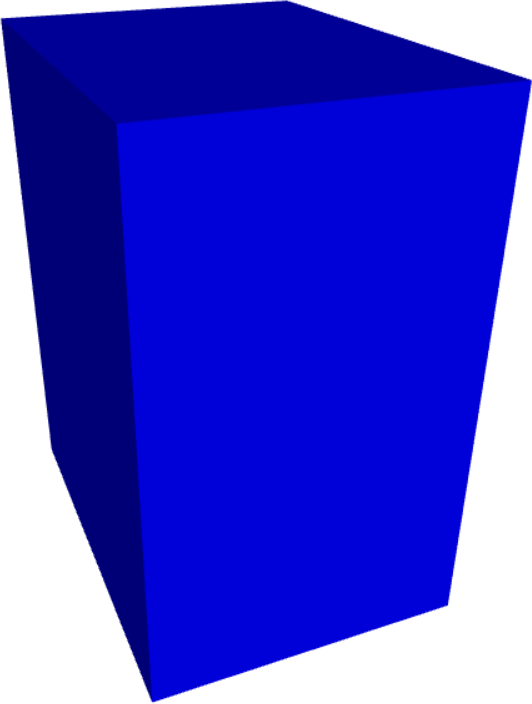
\includegraphics[width=0.3\textwidth]{img/a1-blue-brick.png}
\end{center}
\vspace{-2mm}
\caption{Illustration for Project \ref{2.1}}
\label{fig:a1}
%\vspace{-1cm}
\end{figure}


\subsection{Red Rectangle}\label{2.2}
Create a $3 \times 1$ rectangle in light
red color [200, 0, 0], as shown in Fig. \ref{fig:a2}.\\

\begin{figure}[!ht]
\begin{center}

\includegraphics[width=0.5\textwidth]{img/a2-red-rectangle.png}
\end{center}
\vspace{-2mm}
\caption{Illustration for Project \ref{2.2}}
\label{fig:a2}
\vspace{-0cm}
\end{figure}


\subsection{Orange Octahedron}\label{2.3}
Create an octahedron with vertices 
(0, -1, 1), (0, 1, 1), (0, -1, -1), (0, 1, -1), (2, 0, 0), and (-2, 0, 0). 
Render it using orange color [255, 140, 0]
as shown in Fig. \ref{fig:a3}.

\begin{figure}[!ht]
\begin{center}
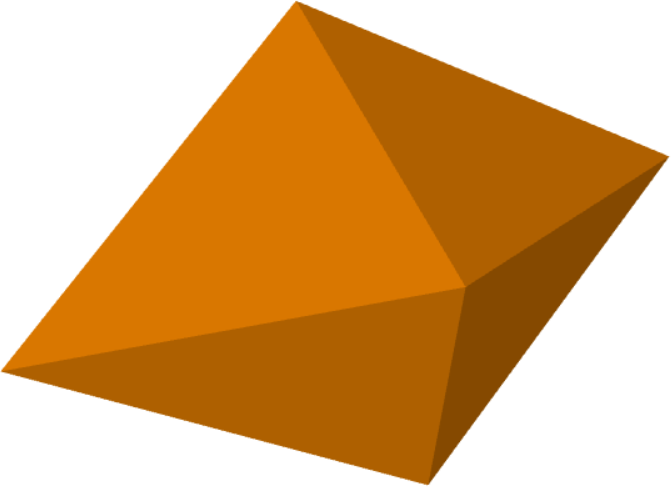
\includegraphics[width=0.3\textwidth]{img/a3-orange-octahedron.png}
\end{center}
\vspace{-2mm}
\caption{Illustration for Project \ref{2.3}}
\label{fig:a3}
%\vspace{-1cm}
\end{figure}




\subsection{Pink Pentagon}\label{2.4}
Create a pentagon with equally-long edges that is inscribed 
in a circle with diameter $R$ and center (0, 0). Render it in pink color [255, 0, 255],
as shown in Fig. \ref{fig:a4}.
\newpage

\begin{figure}[!ht]
\begin{center}
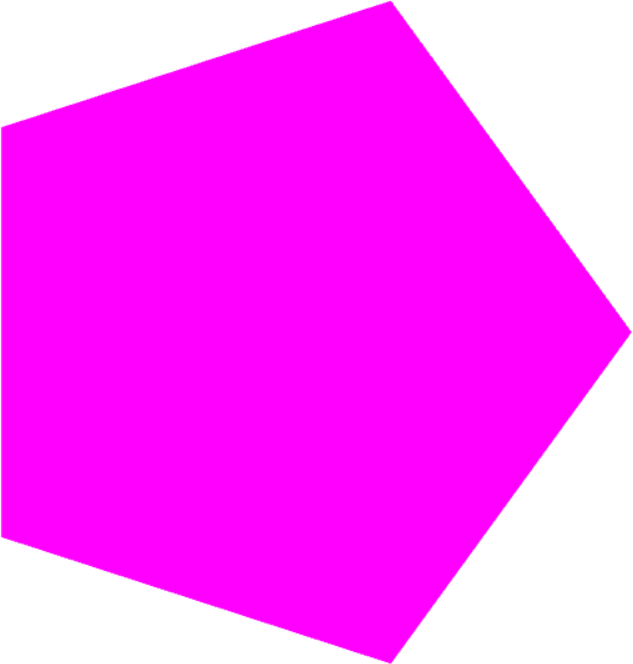
\includegraphics[width=0.3\textwidth]{img/a4-pink-pentagon.png}
\end{center}
\vspace{-4mm}
\caption{Illustration for Project \ref{2.4}}
\label{fig:a4}
\vspace{-4mm}
\end{figure}




\subsection{Cyan Cone}\label{2.5}
Create a cone of radius $R$ and height $H$ that stands on its tip --
the tip is at (0, 0, 0) and the axis of the cone coincides with the 
$z$-axis. Use cyan color [0, 255, 255] as shown in Fig. \ref{fig:a5}.

\begin{figure}[!ht]
\begin{center}

\includegraphics[width=0.3\textwidth]{img/a5-cyan-cone.png}
\end{center}
\vspace{-4mm}
\caption{Illustration for Project \ref{2.5}}
\label{fig:a5}
%\vspace{-1cm}
\end{figure}


\subsection{Carmine Cylinder}\label{2.6}
Create a cylinder of radius $R$ and height $H$.
Render it using carmine color [150, 0, 24]
as shown in Fig. \ref{fig:a6}.
\newpage

\begin{figure}[!ht]
\begin{center}
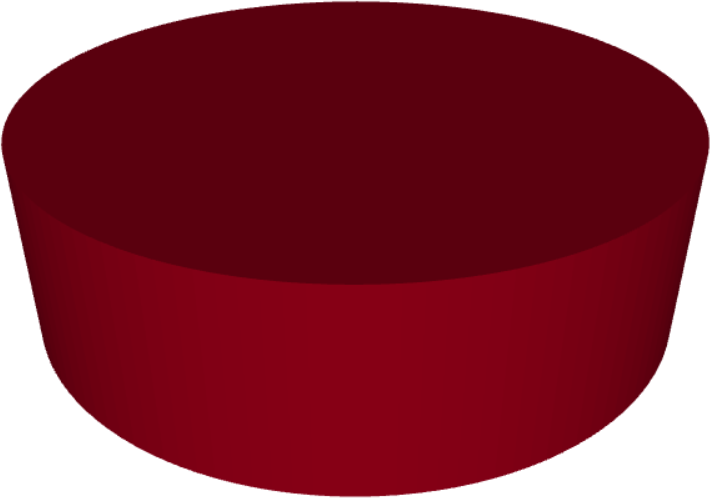
\includegraphics[width=0.3\textwidth]{img/a6-carmine-cylinder.png}
\end{center}
\vspace{-2mm}
\caption{Illustration for Project \ref{2.6}}
\label{fig:a6}
%\vspace{-1cm}
\end{figure}



\subsection{Topaz Tube}\label{2.7}
Create a tube of inner radius $R_{in}$, outer radius $R_{out}$
and height $H$. Render it using topaz color [255, 200, 124]
as shown in Fig. \ref{fig:a7}.

\begin{figure}[!ht]
\begin{center}
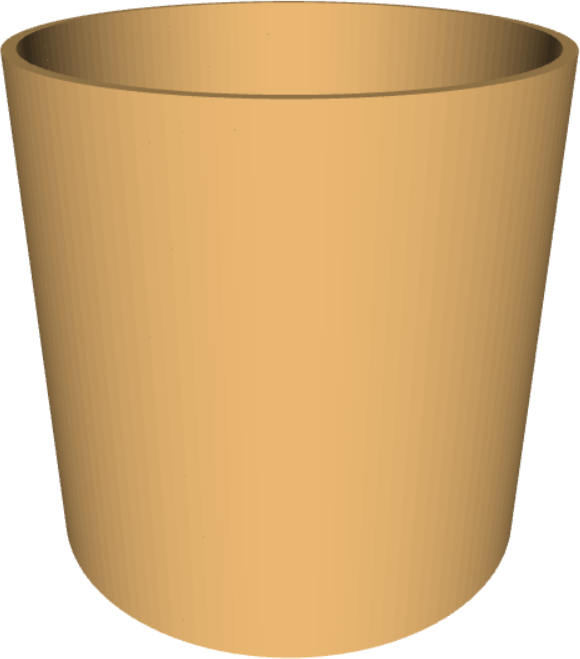
\includegraphics[width=0.3\textwidth]{img/a7-topaz-tube.png}
\end{center}
\vspace{-2mm}
\caption{Illustration for Project \ref{2.7}}
\label{fig:a7}
%\vspace{-1cm}
\end{figure}



\subsection{Sand Sphere}\label{2.8}
Create a sphere of radius $R$ and center at the origin (0, 0, 0). 
Render it using sand color [237, 201, 175]
as shown in Fig. \ref{fig:a8}.
\newpage

\begin{figure}[!ht]
\begin{center}
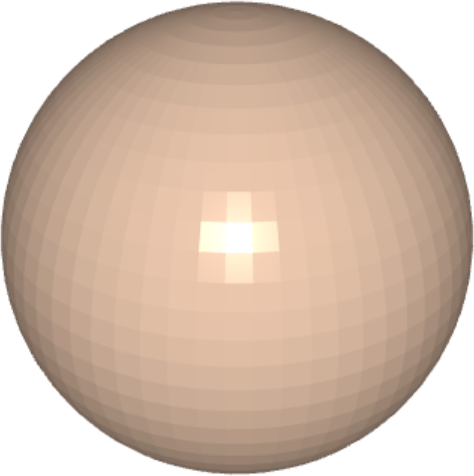
\includegraphics[width=0.3\textwidth]{img/a8-sand-sphere.png}
\end{center}
\vspace{-2mm}
\caption{Illustration for Project \ref{2.8}}
\label{fig:a8}
%\vspace{-1cm}
\end{figure}



\subsection{Turquoise Torus}\label{2.9}
Create a torus of inner radius $R_{in}$ and outer radius $R_{out}$, whose center 
is at the origin (0, 0, 0). The main plane of symmetry should coincide with the 
$xy$-plane. Use turquoise color [64, 224, 208] as shown in Fig. \ref{fig:a9}.


\begin{figure}[!ht]
\begin{center}
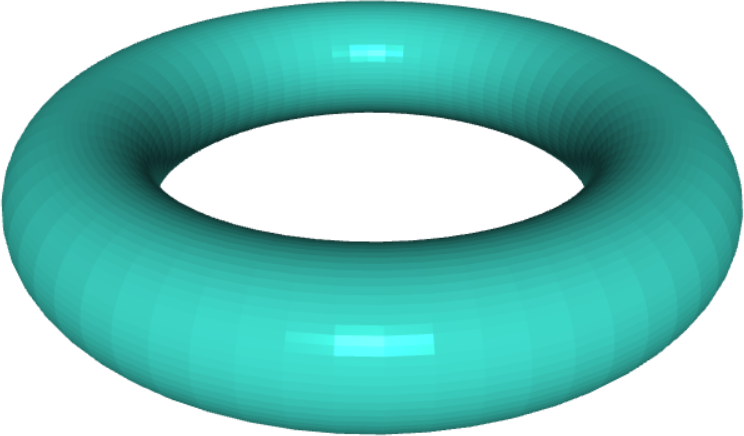
\includegraphics[width=0.5\textwidth]{img/a9-turquoise-torus.png}
\end{center}
\vspace{-2mm}
\caption{Illustration for Project \ref{2.9}}
\label{fig:a9}
%\vspace{-1cm}
\end{figure}



\subsection{Deformed Cylinder}\label{2.10}
Write a script to render a linearly deformed cylinder of radius {\tt R} and height {\tt H}.
The base is a circle of radius {\tt R} and center (0, 0, 0) same as in standard
cylinder. The top circle differs from the standard cylinder -- it is 
shifted by {\tt xshift} and {\tt yshift} in the $x$ and $y$ directions, respectively. 
Render the object using the default grey color [200, 200, 200],
as shown in Fig. \ref{fig:a10}.

\begin{figure}[!ht]
\begin{center}
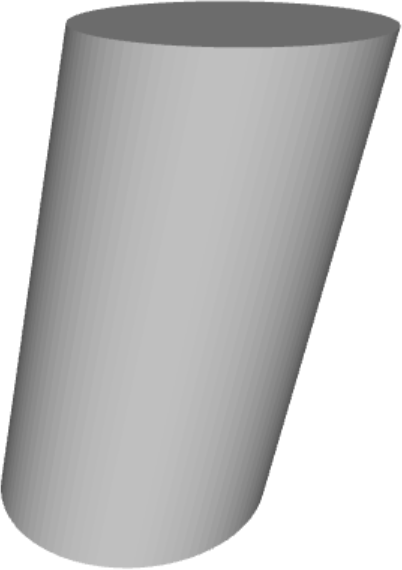
\includegraphics[width=0.3\textwidth]{img/a10-shift.png}
\end{center}
\vspace{-2mm}
\caption{Illustration for Project \ref{2.10}}
\label{fig:a10}
%\vspace{-1cm}
\end{figure}




\section{Basic Transformations}



\subsection{Kitchen Table}\label{3.1}
Create a kitchen table with four square legs. All its measures should be in meters and 
variable: leg width {\tt lw}, leg height {\tt lh}, table measures {\tt ta} and {\tt tb}, and
table thickness {\tt tt}. The legs should be aligned with the corners of the table.
Render it using the color [77, 107, 80], as shown in Fig. \ref{fig:b1}.


\begin{figure}[!ht]
\begin{center}
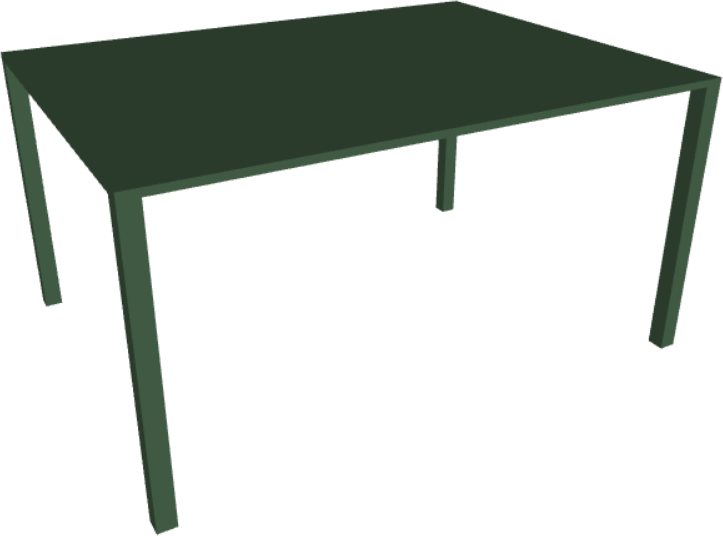
\includegraphics[width=0.3\textwidth]{img/kitchentable.png}
\end{center}
\vspace{-2mm}
\caption{Illustration for Project \ref{3.1}}
\label{fig:b1}
\vspace{-1cm}
\end{figure}
\newpage



\subsection{Tea Table} \label{3.2}
Create a round tea table with four round legs. All of its measures should be 
in meters and variable: leg radius {\tt lr}, leg height {\tt lh}, table radius 
{\tt tr}, table thickness {\tt tt}. The legs should be placed into the 
vertices of a square of size {\tt s} whose center lies at the origin (0, 0).
Render the table using the color [77, 107, 80], as shown in Fig. \ref{fig:b2}.


\begin{figure}[!ht]
\begin{center}
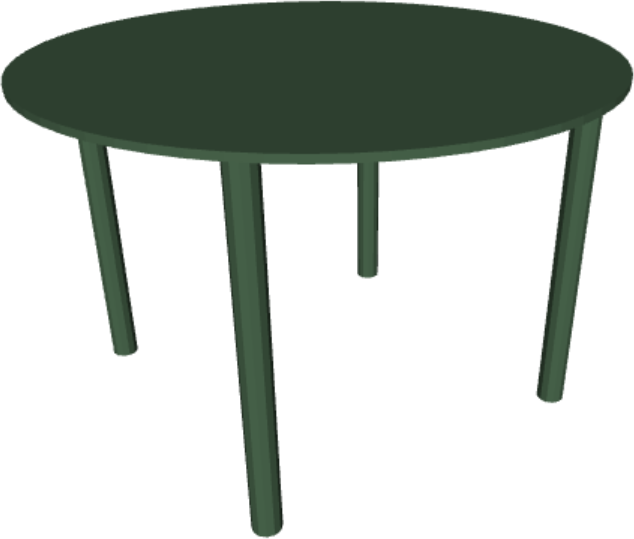
\includegraphics[width=0.3\textwidth]{img/teatable.png}
\end{center}
\vspace{-2mm}
\caption{Illustration for Project \ref{3.2}}
\label{fig:b2}
%\vspace{-1cm}
\end{figure}



\subsection{Padlock} \label{3.3}
Use a scaled cylinder and a torus to create a padlock that is shown in Fig. \ref{fig:b3}. 
All of its measures should be in meters and variable: length and width of the body base 
{\tt ra} and {\tt rb}, body height {\tt h}, top inner radius {\tt rin}
and outer radius {\tt rout}. The arc should be formed by exactly one half of
a torus and placed symmetrically on top of the base. The base should be rendered using 
gold color [212, 175, 55] and the top using silver color [255, 255, 255].

\begin{figure}[!ht]
\begin{center}
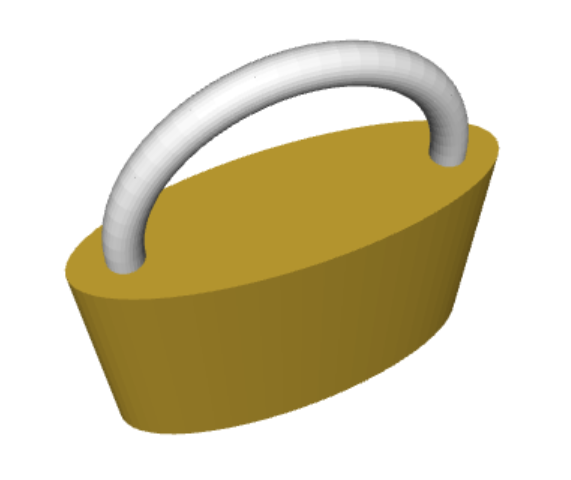
\includegraphics[width=0.3\textwidth]{img/padlock.png}
\end{center}
\vspace{-2mm}
\caption{Illustration for Project \ref{3.3}}
\label{fig:b3}
%\vspace{-1cm}
\end{figure}


\subsection{Bottle} \label{3.4}
Use two cylinders and a sphere to create a simple bottle shown in Fig. \ref{fig:b4}. 
All of its measures should be in meters and variable: base radius {\tt r}, base
cylinder height {\tt bch}, neck radius {\tt rn}, total bottle height {\tt th}.
Render the object using the color [0, 150, 0].

\begin{figure}[!ht]
\begin{center}
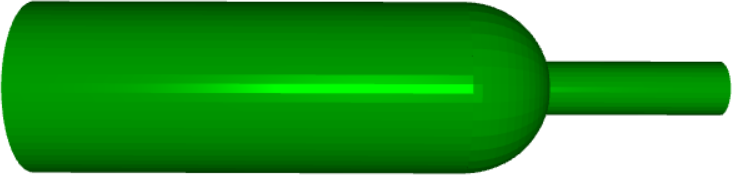
\includegraphics[width=0.5\textwidth]{img/bottle.png}
\end{center}
\vspace{-2mm}
\caption{Illustration for Project \ref{3.4}}
\label{fig:b4}
%\vspace{-1cm}
\end{figure}


\section{Boolean Operations}

\subsection{NCLab icon} \label{4.1}
Cut off parts of a $4 \times 4 \times 4$ brick to create the object shown in 
Fig. \ref{fig:nclabicon}. The cross-section of all parts of the frame is 
a $1 \times 1$ square.


\begin{figure}[!ht]
\begin{center}

\includegraphics[width=0.3\textwidth]{img/nclabicon.png}
\end{center}
\vspace{-2mm}
\caption{Illustration for Project \ref{4.1}}
\label{fig:nclabicon}
%\vspace{-1cm}
\end{figure}
\noindent


\subsection{Drilled Cube} \label{4.2}
Create a cube and drill three holes into it from the three axial 
directions, as illustrated in Fig. \ref{fig:drilledcube}.
The {\tt size} of the cube as well as the {\tt radius} of the 
holes should be in meters and variable. 

\begin{figure}[!ht]
\begin{center}
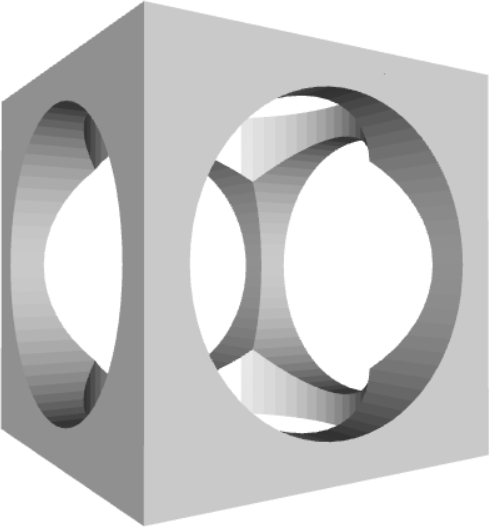
\includegraphics[width=0.3\textwidth]{img/drilledcube.png}
\end{center}
\vspace{-2mm}
\caption{Illustration for Project \ref{4.2}}
\label{fig:drilledcube}
%\vspace{-1cm}
\end{figure}


\subsection{Ashtray} \label{4.3}
Build a simple model of an ashtray using cylindrical shapes, 
as illustrated in Fig. \ref{fig:ashtray}. All measures should be 
in meters and variable: Outer radius {\tt Rout}, inner radius {\tt Rin},
height {\tt Hout}, bottom thickness {\tt bt}, radius of the four 
circular arcs {\tt Rtiny} to carve out on the sides.

\begin{figure}[!ht]
\begin{center}
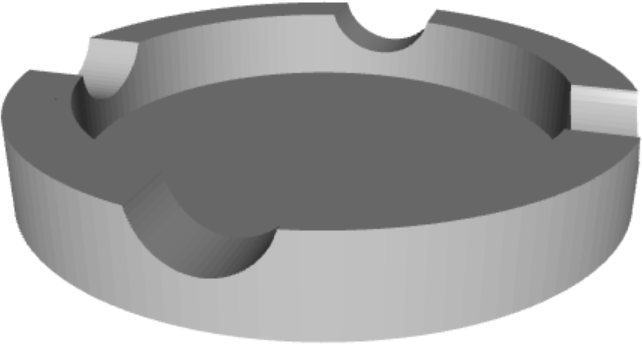
\includegraphics[width=0.3\textwidth]{img/ashtray.png}
\end{center}
\vspace{-2mm}
\caption{Illustration for Project \ref{4.2}}
\label{fig:ashtray}
%\vspace{-1cm}
\end{figure}
\noindent



%\section{Curves and Curved Surfaces}\label{sec:curves}

%\subsection{Coming Soon}


\section{The Power of Scripting}

\subsection{Aztec Pyramid} \label{6.1}
Build an Aztec Pyramid as illustrated in Fig. \ref{fig:aztec}. All measures should be 
in meters and variable: length 
on the bottom side {{\tt BSL}}, length of the top side {\tt TSL}, 
height {\tt H}, and the number of layers {\tt N}. Your script should 
detect if the user's parameters are incorrect (such as if one of the lengths is negative or 
zero) and print an error message.


\begin{figure}[!ht]
\begin{center}
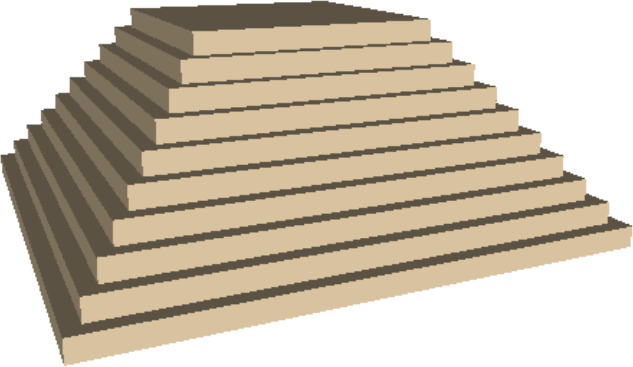
\includegraphics[width=0.5\textwidth]{img/aztec.png}
\end{center}
\vspace{-2mm}
\caption{Illustration for Project \ref{6.1}}
\label{fig:aztec}
%\vspace{-1cm}
\end{figure}
\noindent



\subsection{Towers of Hanoi} \label{6.2}
Build a model of the Towers of Hanoi game as illustrated in Fig. \ref{fig:hanoi}. 
The number of discs, radius of the largest and smallest disc, and the height of the tower 
should be user-defined parameters. The base and poles should have the color of wood
[184, 115, 51] while the discs should have random colors.


\begin{figure}[!ht]
\begin{center}
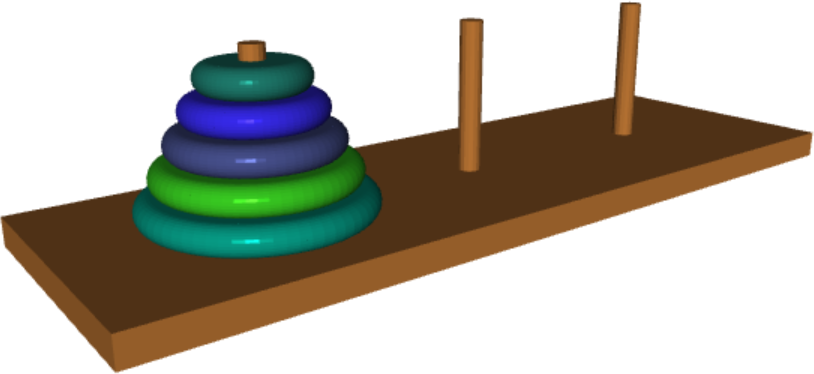
\includegraphics[width=0.5\textwidth]{img/hanoi.png}
\end{center}
\vspace{-2mm}
\caption{Illustration for Project \ref{6.2}}
\label{fig:hanoi}
%\vspace{-1cm}
\end{figure}
\noindent


\subsection{Horse Corral} \label{6.3}
Build a polygonal horse corral with $N$ equally-long sides that are inscribed into a circle with radius $r$.
The poles should have general user-defined dimensions $W \times W \times H$. Fig. \ref{fig:corral2} shows 
how the corral should look like for $N = 8$.

\begin{figure}[!ht]
\begin{center}
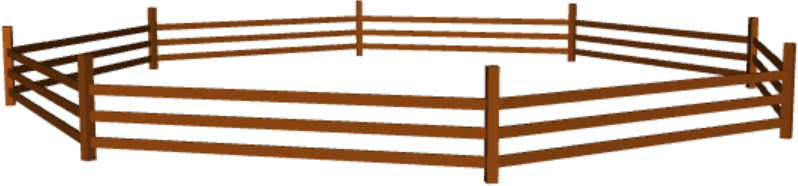
\includegraphics[width=0.5\textwidth]{img/tam-3.png}
\end{center}
\vspace{-2mm}
\caption{Illustration for Project \ref{6.3}}
\label{fig:corral2}
%\vspace{-1cm}
\end{figure}
\noindent


\subsection{Wagon Wheel} \label{6.4}
Build a spoked wagon wheel similar to the one in Fig. \ref{fig:wheel-1}. All radiuses 
and thicknesses should be user-defined, as well as the number of spokes.


\begin{figure}[!ht]
\begin{center}
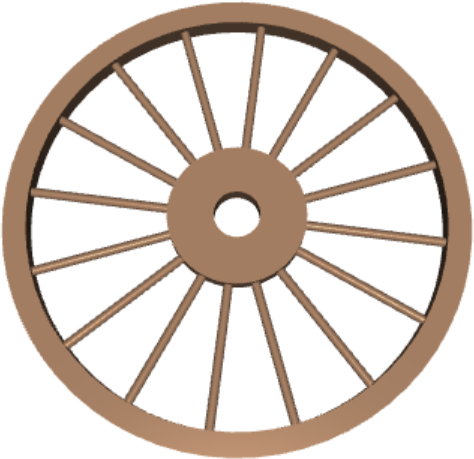
\includegraphics[width=0.3\textwidth]{img/wagonwheel-1.png}
\end{center}
\vspace{-4mm}
\caption{Illustration for Project \ref{6.4}}
\label{fig:wheel-1}
%\vspace{-1cm}
\end{figure}
\noindent

